\chapter{Background}
\label{chap:background}

\section{Introduction to Fundamental Concepts}
Modern cybersecurity faces increasingly sophisticated threats, particularly Advanced Persistent Threats (APTs). When 900 companies were surveyed about the most likely attacks on their business, APTs ranked at 57\% \cite{aag2024stats}. These threats require structured analysis frameworks to be understood and countered. The emergence of Machine Learning (ML) has introduced new dynamics and perspectives, serving both as a powerful tool for attackers to automate and personalize their operations, and for defenders to improve early detection and incident response. This chapter lays the conceptual foundations by examining these three essential pillars (APT, framework, ML) that support the development of an ML-augmented framework for detecting multi-stage APT attacks.

\section{Overview of Cybersecurity}

\subsection{Definition and Scope of Cybersecurity}
Cybersecurity is defined as the practice of protecting systems, networks, programs, and data from digital attacks, unauthorized access, damage, or destruction~\cite{cains2022cybersecurity,nist2023cyber}. It include a broad set of technologies, processes, and practices designed to defend information assets across all layers of a digital environment --- from hardware infrastructure to software applications and human behavior~\cite{cisco2024cyber}.

The scope of cybersecurity extends across multiple domains, each addressing a distinct layer of protection~\cite{kang2023zero,cynet2023basics}:
\begin{itemize}
    \item \textbf{Network Security}: Protecting the integrity and usability of network infrastructure by preventing unauthorized access, misuse, or denial of service attacks.
    \item \textbf{Endpoint Security}: Securing individual devices such as computers, smartphones, and servers that connect to a network and serve as entry points for threats.
    \item \textbf{Application Security}: Ensuring that software applications are designed, developed, and maintained to resist exploitation of vulnerabilities.
    \item \textbf{Data Security}: Protecting the confidentiality, integrity, and availability of data --- whether stored, processed, or transmitted --- from unauthorized access or corruption.
    \item \textbf{Identity and Access Management (IAM)}: Controlling who has access to which resources, ensuring that only authorized users can interact with sensitive systems.
    \item \textbf{Cloud Security}: Addressing the unique risks of cloud environments, including misconfiguration, data breaches, and insecure interfaces.
    \item \textbf{Operational Security (OpSec)}: Managing the processes and decisions around handling and protecting data assets, including user behavior and access permissions.
\end{itemize}

\customexplication{A useful analogy is to think of cybersecurity as a multi-layered defense system --- similar to a medieval castle. The outer walls (network security) , the guards (endpoint and identity management) verify who enters, the vault (data security) .}

The field is commonly structured around three foundational principles, collectively known as the CIA Triad:
\begin{itemize}
    \item \textbf{Confidentiality}: Ensuring that information is accessible only to those authorized to access it.
    \item \textbf{Integrity}: Ensuring that data is accurate, consistent, and has not been tampered with.
    \item \textbf{Availability}: Ensuring that systems and data are accessible to authorized users when needed.
\end{itemize}

These three principles --- Confidentiality, Integrity, and Availability --- serve as the evaluation criteria for nearly every security control and framework discussed throughout this document, including STRIDE, the Cyber Kill Chain, and MITRE ATT\&CK.
\clearpage
As cyber threats have grown in sophistication, the scope of cybersecurity has expanded beyond purely technical concerns. Modern cybersecurity must address not only technological vulnerabilities, but also human factors such as social engineering, insider threats, and security awareness~\cite{chandel2017social}. This general view --- covering people, processes, and technology --- forms the foundation upon which advanced threat detection and response strategies, such as those discussed in subsequent sections, are built.

\subsection{Key Cybersecurity Concepts and Terminology}
A solid understanding of cybersecurity requires familiarity with its core vocabulary. The following concepts are foundational and appear throughout the literature, frameworks, and detection methodologies discussed in this document.

\begin{itemize}
      \item \textbf{Asset}: Any resource of value to an organization --- including hardware, software, data, networks, and personnel --- that must be protected from threats~\cite{hentea2021risk,huntress2024glossary}.
      \item \textbf{Threat}: Any potential event or action that could exploit a vulnerability to cause harm to an asset~\cite{huntress2024glossary}. Threats can be intentional (malicious attackers) or unintentional (human error, natural disasters).
      \item \textbf{Vulnerability}: A weakness or flaw in a system, application, or process that can be exploited by a threat actor. Vulnerabilities may exist in software code, system configurations, or organizational procedures~\cite{hentea2021risk}.
    \item \textbf{Exploit}: A specific method, tool, or piece of code that takes advantage of a vulnerability to cause unintended or unauthorized behavior in a system.
    \item \textbf{Risk}: The potential for loss or damage when a threat successfully exploits a vulnerability. Risk is commonly expressed as:
    \begin{center}
        $Risk = Threat \times Vulnerability \times Impact$
    \end{center}
      \item \textbf{Attack Surface}: The total sum of all possible entry points --- or attack vectors --- through which an unauthorized user could attempt to enter or extract data from a system. The larger the attack surface, the greater the exposure to potential threats~\cite{sentinelone2024vector}.
      \item \textbf{Attack Vector}: The specific path or method used by an attacker to gain unauthorized access to a system. Common vectors include phishing emails, unpatched software, weak passwords, and misconfigured cloud services~\cite{sentinelone2024vector}.
    \item \textbf{Threat Actor}: Any individual, group, or entity responsible for a security incident or attack. Threat actors are typically categorized by their motivation and capability:
    \begin{itemize}
        \item \textit{Nation-State Actors}: Highly skilled, state-sponsored groups conducting espionage or sabotage (e.g., APT groups).
        \item \textit{Cybercriminals}: Financially motivated individuals or organized groups.
        \item \textit{Insider Threats}: Employees or contractors who misuse their access, intentionally or accidentally.
        \item \textit{Hacktivists}: Groups motivated by political or ideological goals.
    \end{itemize}
\item \textbf{Indicator of Compromise (IoC)}: Evidence that a system has been breached or is under attack~\cite{crowdstrike2024ioa}. Common IoCs include unusual network traffic, unexpected file changes, unfamiliar processes, or suspicious login activity.
      \item \textbf{Indicator of Attack (IoA)}: Unlike IoCs --- which detect a breach after it occurs --- IoAs focus on detecting the behavior of an attack in progress, enabling earlier intervention before significant damage is done~\cite{crowdstrike2024ioa}.
\end{itemize}


\begin{itemize}
      \item \textbf{Payload}: The component of malicious software (malware) that executes the intended malicious action --- such as encrypting files, stealing credentials, or establishing a backdoor \footnote{backdoor is a hidden way to get into a system bypassing normal security (like login, authentication)} --- once delivered to a target system~\cite{cloudflare2024payload}.
      \item \textbf{Zero-Day Vulnerability}: A software flaw that is unknown to the vendor and for which no patch or fix yet exists at the time of exploitation~\cite{deepinstinct2023zeroday}. Zero-day vulnerabilities are highly valuable to advanced threat actors, including APT groups, precisely because they cannot be detected by signature-based security systems \footnote{Signature-based security systems detect threats by comparing observed events against a database of known malicious patterns or ``signatures''.}.
\end{itemize}

\customnote{The Stuxnet attack --- referenced in Section 1.3 --- is one of the most documented examples of zero-day exploitation in history, relying on four simultaneous zero-day vulnerabilities to compromise its target.}

\begin{itemize}
      \item \textbf{Lateral Movement}: The techniques used by an attacker --- after gaining initial access to a network --- to progressively move through systems and gain access to higher-value targets~\cite{crowdstrike2024ioa}. Lateral movement is a defining characteristic of APT attacks and is further detailed in Sections 1.3 and 1.5.
      \item \textbf{Persistence}: The ability of an attacker to maintain long-term, undetected access to a compromised system, even after reboots or credential changes. Attackers achieve persistence through backdoors, scheduled tasks, or registry modifications.
      \item \textbf{Defense in Depth}: A layered security strategy that deploys multiple, overlapping security controls so that if one layer fails, others remain in place to prevent or detect an attack~\cite{cloudflare2024defense}. This principle underlies the multi-framework approach --- combining CKC, MITRE ATT\&CK, and Machine Learning --- explored throughout this document, as shown in Figure~\ref{fig:defense_in_depth}.
\end{itemize}

\begin{figure}[H]
    \centering
    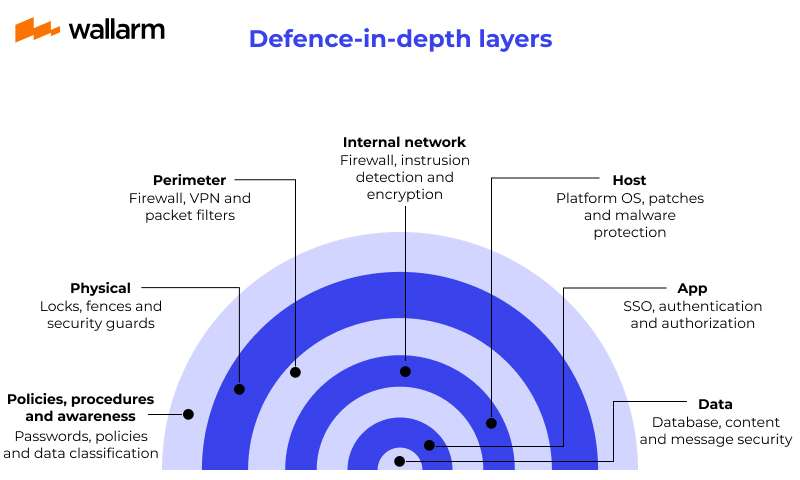
\includegraphics[width=0.8\textwidth]{figures/ch1/defense.jpeg}
    \caption{Illustration of the Defense in Depth security strategy.}
    \label{fig:defense_in_depth}
\end{figure}

\subsection{Major Categories of Cyber Threats}
Cyber threats manifest in many forms, each with distinct mechanisms, objectives, and levels of sophistication. Understanding these categories is essential for designing effective detection and mitigation strategies. The following classification covers the most common  threat types encountered in modern cybersecurity environments~\cite{enisa2023threats}.

\textbf{Malware}\par
Malware (malicious software) is any software intentionally designed to disrupt, damage, or gain unauthorized access to a system. It represents one of the most common and diverse categories of cyber threats, and includes several subcategories:
\begin{itemize}
    \item \textbf{Viruses}: Malicious code that attaches itself to legitimate programs and spreads when executed.
    \item \textbf{Worms}: Self-replicating malware that spreads across networks without requiring user interaction.
    \item \textbf{Trojans}: Malicious programs disguised as legitimate software to deceive users into executing them.
    \item \textbf{Ransomware}: Malware that encrypts victim data and demands payment for the decryption key.
    \item \textbf{Spyware}: Software that secretly monitors user activity and exfiltrates sensitive information.
    \item \textbf{Rootkits}: Tools designed to hide the presence of malware or unauthorized access from detection systems.
\end{itemize}

\textbf{Social Engineering}\par
Social engineering attacks exploit human psychology rather than technical vulnerabilities, manipulating individuals into revealing confidential information or performing actions that compromise security~\cite{sentinelone2024social,akram2025social}. Key techniques include:
\begin{itemize}
    \item \textbf{Phishing}: Mass distribution of fraudulent emails designed to trick recipients into revealing credentials or clicking malicious links.
    \item \textbf{Spear Phishing}: A highly targeted form of phishing customized  to a specific individual or organization using personalized information.
    \item \textbf{Vishing}: Voice-based social engineering conducted via phone calls.
    \item \textbf{Pretexting}: Creating a fabricated scenario to manipulate a victim into providing information or access.
\end{itemize}

\customexplication{scenario: A cybercriminal first sends a mass email to thousands of employees claiming their account will be suspended � a classic phishing attempt. One employee, Sarah, a senior financial officer, ignores it. The attacker then researches Sarah on LinkedIn and sends her a personalized email referencing her recent project and her manager's name, tricking her into clicking a malicious link � this time using spear phishing. Hours later, Sarah receives a phone call from someone pretending to be IT support, warning her of "suspicious activity" on her account and asking her to confirm her password � a vishing attack ,Finally, the attacker calls the company's front desk, pretending to be a bank employee doing a regular check-up, and convinces the receptionist to share internal contact details � completing the attack through pretexting.}


\textbf{Denial of Service (DoS) and Distributed Denial of Service (DDoS)}\par
These attacks aim to make a system, service, or network unavailable to its  users by overwhelming it with a flood of illegitimate requests~\cite{paloalto2024dos}. In a DDoS attack, this traffic originates from a large number of compromised devices (a botnet), making it significantly harder to mitigate. The targeted security property is Availability --- one of the three pillars of the CIA Triad.

\vspace{1em}
\textbf{Man-in-the-Middle (MitM) Attacks}\par
In a MitM attack, the attacker secretly intercepts and potentially alters communication between two parties who believe they are communicating directly with each other~\cite{hussain2023mitm,rapid72024mitm}. This allows the attacker to spy, steal credentials, or inject malicious content into the communication stream without either party's knowledge.

\vspace{1em}
\textbf{Insider Threats}\par
Insider threats originate from individuals within the organization --- such as employees, contractors, or business partners --- who misuse their authorized access to harm the organization. They are categorized as:
\begin{itemize}
    \item \textbf{Malicious Insiders}: Individuals who intentionally abuse their access for personal gain, espionage, or sabotage.
    \item \textbf{Negligent Insiders}: Users who unintentionally cause security incidents through careless behavior, such as clicking phishing links or mishandling sensitive data.
\end{itemize}

\textbf{Supply Chain Attacks}\par
Supply chain attacks target less-secure elements within a software or hardware supply chain to compromise a final, higher-value target. Rather than attacking an organization directly, the adversary infiltrates a trusted third-party vendor, software update mechanism, or component manufacturer to gain indirect access. Notable examples include the SolarWinds attack (2020), in which a compromised software update was distributed to thousands of organizations worldwide.

\textbf{Advanced Persistent Threats (APT)}\par
APTs represent the most sophisticated category of cyber threats. Unlike other attack types that seek immediate gains, APTs are characterized by stealth, persistence, and long-term strategic objectives --- such as espionage, sabotage, or data exfiltration~\cite{krishnapriya2024comprehensive}. APTs are typically conducted by nation-state actors or highly organized criminal groups with significant resources~\cite{crowdstrike2024apt}.

\customnote{Because APTs combine multiple threat categories --- malware, social engineering, lateral movement, and zero-day exploitation --- into a coordinated, multi-stage campaign, they require dedicated detection frameworks beyond standard security tools. This is precisely why Chapter 1 dedicates the following sections entirely to APT modeling, detection frameworks, and Machine Learning-based countermeasures.}

The taxonomy above illustrates that cyber threats vary greatly in complexity, origin, and intent. While traditional security tools are effective against known, lower-sophistication threats such as common malware and phishing, they fall short when facing multi-stage, adaptive attacks like APTs. This limitation motivates the adoption of structured frameworks and intelligent detection methods --- which form the core focus of this document.

\section{Advanced Persistent Threats (APT)}
\subsection{Definition and Characteristics}
The term \textbf{Advanced Persistent Threat (APT)} was introduced in 2006 by analysts at the United States Air Force (USAF) to describe intrusion activities that possessed specific characteristics \cite{singh2016comprehensive}. An APT is a targeted cyberattack that gains illegal access to information and communication systems with the aim of infiltrating and exfiltrating confidential data or harming an enterprise \cite{krishnapriya2024comprehensive}.

APTs are distinguished from traditional cybercriminal attacks by three main characteristics \cite{krishnapriya2024comprehensive,singh2016comprehensive}:
\begin{enumerate}
    \item \textbf{Advanced}: Attackers use sophisticated tools and techniques to bypass detection systems and maintain access to well-protected networks. The hacker is usually well-organized, adaptive in nature, and possesses significant resources \cite{singh2016comprehensive}.
    \item \textbf{Persistent}: The attacker demonstrates strong determination towards their target, using a slow process extended over time to achieve their objective. Persistence involves constantly collecting data from the target by exploiting various vulnerabilities \cite{krishnapriya2024comprehensive}. Even if the attacker achieves their initial goal, they persist within the system for further data exfiltration or to execute other significant changes.
    \item \textbf{Threat}: The attacker possesses the capability to access information, and the goal of the attack is often motivated by strategic advantages, industrial, military, or economic espionage, or political manipulation, rather than simple quick financial gains \cite{singh2016comprehensive}.
\end{enumerate}

\customexplication{As an analogy, consider two burglars: a direct attacker steals everything at once, ensuring immediate discovery. Conversely, an APT attacker discreetly copies the house key and secretly returns over time to steal small items sequentially. The key difference is the APT attacker's undetected persistence.}

The dwell time\footnote{Dwell time refers to the duration a cyber attacker remains undetected within a compromised network.} of APTs is often very long, highlighting the difficulty current detection systems have in identifying these stealthy attacks \cite{krishnapriya2024comprehensive}. APTs are generally implemented in several stages, often referred to as ``slow poisoning'' \cite{krishnapriya2024comprehensive}. They employ Tools, Techniques, and Procedures (TTPs) that are often novel and specifically developed to evade signature-based security systems For example, the Stuxnet attack was particularly complex and remarkable because it relied on four zero-day vulnerabilities simultaneously, digital signature forgeries, and deep knowledge of the target environment \cite{singh2016comprehensive}.

\customnote{The Stuxnet attack will be discussed in detail during the historical section of the ``Future Trends in Cyber Attacks'' chapter.}

\begin{figure}[H]
    \centering
    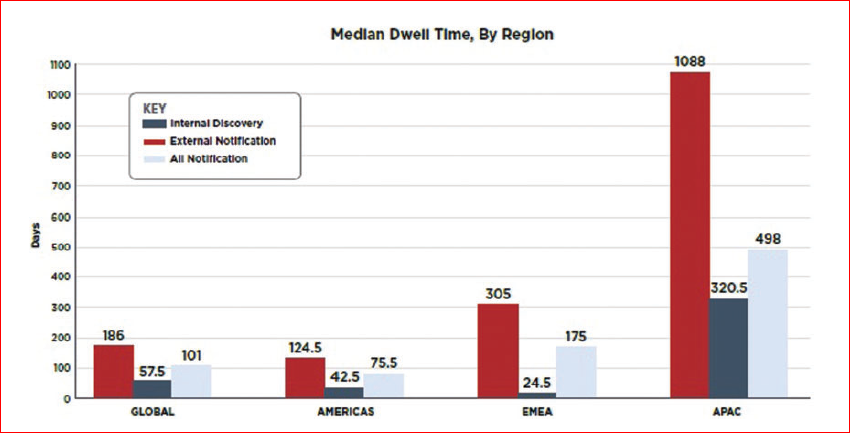
\includegraphics[width=0.7\textwidth]{figures/ch1/dwell}
    \caption{Dwell time in APT attacks}
    \label{fig:dwell}
\end{figure}

\subsection{Modeling APT Phases}
The APT attack process is inherently multi-stage. Although the exact number of steps may vary (some models describe four, five, six, or even eight), a typical APT lifecycle includes five essential phases for the majority of attacks \cite{krishnapriya2024comprehensive}:
\begin{enumerate}
    \item \textbf{Information Gathering (Reconnaissance)}: The attacker gathers information about the target organization, its resources, employees, and relationships, often via social engineering and passive web tools \cite{krishnapriya2024comprehensive}. This phase is crucial for developing attack tools and identifying the weakest link \cite{singh2016comprehensive}.
    \item \textbf{Initial Intrusion}: The adversary establishes a Point of Entry (POE) using social engineering techniques like \textbf{spear-phishing} (malicious email or link), water-hole attacks, or software vulnerability exploitation, often involving malware execution \cite{krishnapriya2024comprehensive}. Spear-phishing is the most commonly used technique for initial intrusion \cite{singh2016comprehensive}.
    \item \textbf{Command and Control (C\&C)}: A covert communication channel is established between the compromised host(s) and an external C\&C server. This communication must be maintained until the end of the attack and is essential for data transfer \cite{krishnapriya2024comprehensive}.
    \item \textbf{Lateral Movement}: The attacker attempts to move through the network by infecting more devices until reaching high-value targets, often using legitimate tools or reusing stolen credentials (credential dumping, pass-the-hash) \cite{krishnapriya2024comprehensive}.
    \item \textbf{Action on Objectives (AoO)}: The attacker achieves their ultimate goal, which may be data exfiltration, financial theft, system alteration (as in Stuxnet), or data destruction \cite{krishnapriya2024comprehensive}.
\end{enumerate}

\customwarning{It is important to note that different authors and experts may model APT phases differently. For example, some sources divide the attack into: Reconnaissance, Breach, Infiltration, Exfiltration, and Stealth Persistence. Because of these varying perspectives, the cybersecurity community emphasizes the need for standardized frameworks to provide a unified point of view.}

\begin{figure}[H]
    \centering
    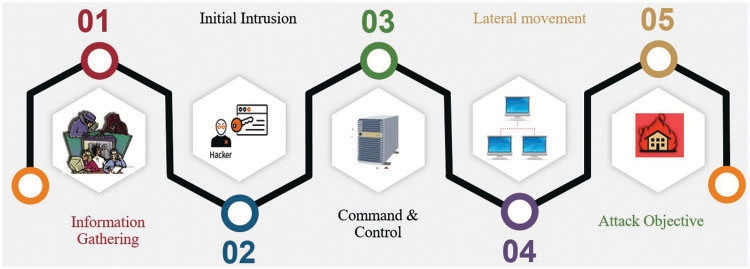
\includegraphics[width=0.8\textwidth]{figures/ch1/apt_steps}
    \caption{Stages of an APT attack}
    \label{fig:apt_steps}
\end{figure}

\section{Introduction to Threat Modeling Frameworks}

While the terms are often used as if they mean the same thing, there are actually three distinct categories of conceptual models used in cybersecurity. Each serves a different purpose in analyzing, classifying, and mitigating cyber threats� that is, taking protective measures to reduce, limit, or prevent the damage that cyber threats can cause. \cite{tatam2021review, huang2024security}.

\subsection{Category 1: Attack Lifecycle Models}
These models describe the stages of how an attack unfolds from start to finish \cite{tatam2021review, huang2024security}.
\begin{itemize}
    \item \textbf{Cyber Kill Chain:} Created by Lockheed Martin (2011), it outlines the 7 stages of an attack from reconnaissance to the final objective. It is formally defined as: reconnaissance, weaponization, delivery, exploitation, installation, command and control (C2), and actions on objectives (AoO) \cite{tatam2021review}.
    \item \textbf{MITRE ATT\&CK:} Created by MITRE (2013), it details the tactics and techniques of real attackers based on real-world incidents \cite{jiang2025mitre, tatam2021review}. Organized into three technology domains---Enterprise (traditional networks and cloud technologies), Mobile (mobile devices), and ICS (Industrial Control Systems)---it maps specific adversarial tactics (high-level objectives) and techniques (specific actions) that describe how an attacker seeks to compromise or persist in a system \cite{jiang2025mitre}.
    \item \textbf{Unified Kill Chain:} Created by Paul Pols (2017), this is an extended version that includes  18 phases, offering more detail than the traditional Kill Chain. It was developed by combining and extending the Cyber Kill Chain with the MITRE ATT\&CK framework \cite{tatam2021review}.
\end{itemize}

\customnote{The Cyber Kill Chain and the MITRE ATT\&CK framework will be discussed in detail in different sub-parts, as they represent the core of threat detection methods and are some of the most widely used frameworks.}

\subsection{Category 2: Threat Modeling Frameworks}
These frameworks help security professionals analyze and classify threats during the system design phase \cite{huang2024security, ouaissa2025smartcity}. Threat modeling is a proactive approach used primarily in the early stages of a system's lifecycle to anticipate potential cybersecurity threats and vulnerabilities, enabling the incorporation of relevant mitigation controls into the system design \cite{huang2024security, owasp2024threatmodeling}.
\begin{itemize}
    \item \textbf{STRIDE:} Classifies threats into 6 types: Spoofing, Tampering, Repudiation, Information Disclosure, Denial of Service (DoS), and Elevation of Privilege. First introduced to developers at Microsoft in 1999, STRIDE is a system/software-based taxonomy for identifying threats based on their explicit type \cite{tatam2021review, ouaissa2025smartcity}.
    \item \textbf{PASTA:(Process for Attack Simulation and Threat Analysis)}a seven-step threat modeling methodology that integrates business objectives and technical requirements to deliver a comprehensive, risk-based assessment of potential threats. Unlike other methodologies focused exclusively on technical vulnerabilities, PASTA let's you adopts  the whole approach that considers both business impact and technological concerns \cite{ouaissa2025smartcity}.
    
    \begin{figure}[H]
        \centering
        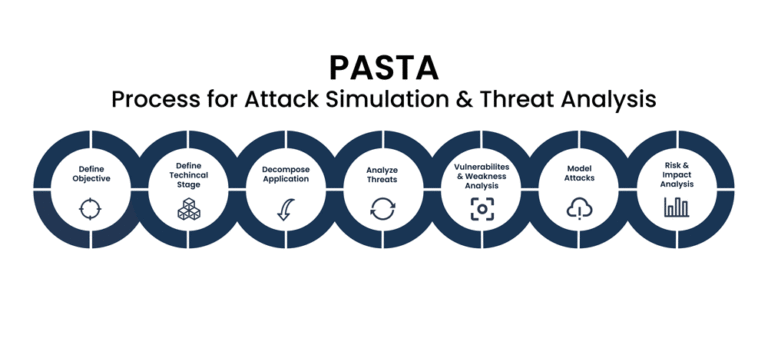
\includegraphics[width=0.7\textwidth]{figures/ch1/PASTA.png}
        \caption{Steps of the PASTA methodology}
        \label{fig:pasta}
    \end{figure}

    \item \textbf{DREAD:} Rates threats by 5 categories: Damage potential, Reproducibility, Exploitability, Affected users, and Discoverability. Initially established as part of Microsoft's Security Development Lifecycle (SDL), it has since become a widely adopted approach for risk prioritization across a variety of sectors \cite{ouaissa2025smartcity}.
    \item \textbf{VAST:} Built specifically for large-scale enterprises and agile/DevOps environments, it provides a scalable threat modeling approach suitable for complex organizational contexts \cite{tatam2021review, ouaissa2025smartcity}.
    \item \textbf{Attack Trees:} A visual tree structure mapping all possible paths to achieve an attack goal. Attack Trees formally identify and define the variety of attacks a system can be subjected to, representing them in a hierarchical structure where the root node signifies the attacker's goal and the leaf nodes depict all possible paths to fulfill that objective \cite{tatam2021review}.
    
    \begin{figure}[H]
        \centering
        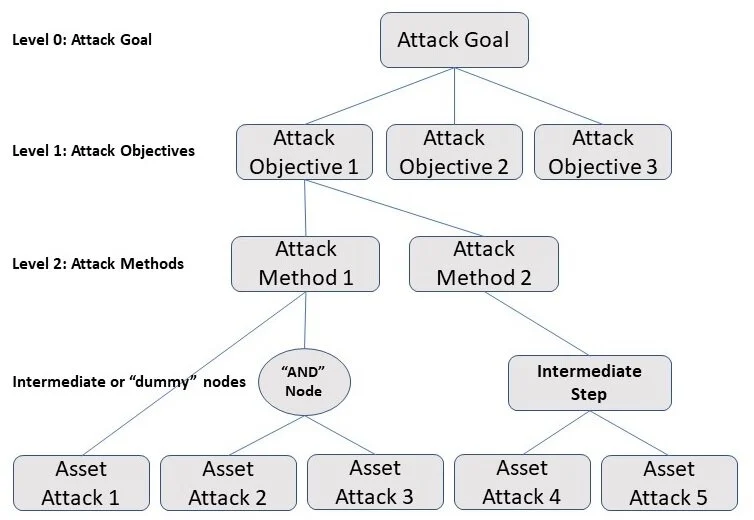
\includegraphics[width=0.7\textwidth]{figures/ch1/tree-attack.png}
        \caption{Example of an Attack Tree structure}
        \label{fig:attack_tree}
    \end{figure}
\end{itemize}

\subsection{Category 3: Adversary Behavior \& Incident Analysis Models}
These models focus on understanding who the attacker is, how they operate, and assisting in incident analysis \cite{tatam2021review, huang2024security}.
\begin{itemize}
    \item \textbf{Diamond Model:} Focuses on the interaction between four fundamental elements: adversary, victim, infrastructure, and capabilities. It is widely used to track attack groups and model intrusion flows. \cite{tatam2021review, huang2024security}.
    \item \textbf{MITRE D3FEND:} The defensive counterpart to ATT\&CK, which maps defensive countermeasures to attack techniques. D3FEND has been integrated with ATT\&CK-based defense strategies, for example against IoT botnet attacks within smart city environments, showcasing the practical utility of combining MITRE offensive and defensive frameworks \cite{jiang2025mitre}.
    \item \textbf{TIBER-EU:} A European framework designed for simulating real Advanced Persistent Threat (APT) attacks on financial institutions, providing a structured methodology for red-team testing and threat intelligence-led adversarial simulations in the financial sector.
\end{itemize}

\customexplication{Each framework category acts as a specific tool serving a distinct phase of the attack timeline. Pre-incident, Category 2 (Threat Modeling) is used to design resilient systems that are not easily bypassed. During an incident, Category 1 (Attack Lifecycle) serves to trace and detect the stages of an active attack. Finally, post-incident, Category 3 (Adversary Behavior) is essential for investigating the attack and profiling the attacker's methods.}

\section{The Cyber Kill Chain (CKC)}
\subsection{Structure and Objective of the Model}
The Cyber Kill Chain (CKC), developed by Lockheed Martin, is a conceptual framework that describes the sequence of steps typically followed by cyber intruders to achieve their goal \cite{singh2016comprehensive, ahmed2021cyber}. This model helps cybersecurity professionals identify and mitigate threats by decomposing the attack lifecycle into discrete phases, allowing for more targeted and effective defense measures. The CKC model has been widely used to analyze APT campaigns, providing a taxonomy based on the adversary's TTPs \cite{jiang2025mitre, ahmed2021cyber}.

\subsection{Detailed Description of the Seven Phases}
The CKC model consists of seven distinct stages, the execution of which in an uninterrupted sequence is necessary for the success of the attack \cite{singh2016comprehensive, ahmed2021cyber}:
\begin{enumerate}
    \item \textbf{Reconnaissance}: The attacker performs research on the target to identify systems, employees, and exploitable vulnerabilities \cite{krishnapriya2024comprehensive}.
    \item \textbf{Weaponization}: The attacker couples malware (such as a Remote Access Trojan - RAT) with an exploit code (exploit kit) into a deliverable payload, such as PDF or Microsoft Office files \cite{singh2016comprehensive}.
    \item \textbf{Delivery}: The payload is transmitted to the target, often via email (phishing), compromised websites, or removable media \cite{singh2016comprehensive}.
    \item \textbf{Exploitation}: Once the payload is successfully delivered, a vulnerability is exploited to execute malicious code on the target system \cite{singh2016comprehensive}.
    \item \textbf{Installation}: The attacker installs persistent access points (e.g., backdoors or persistence mechanisms) to guarantee continuous access to the system or network \cite{singh2016comprehensive}.
    \item \textbf{Command and Control (C\&C)}: The adversary establishes a communication channel with the compromised host to manipulate the cyber weapon and guide actions remotely \cite{krishnapriya2024comprehensive}.
    \item \textbf{Action on Objectives (AoO)}: The attacker realizes their final objective, such as data theft, encryption, or information destruction \cite{krishnapriya2024comprehensive}.
\end{enumerate}

\begin{figure}[H]
    \centering
    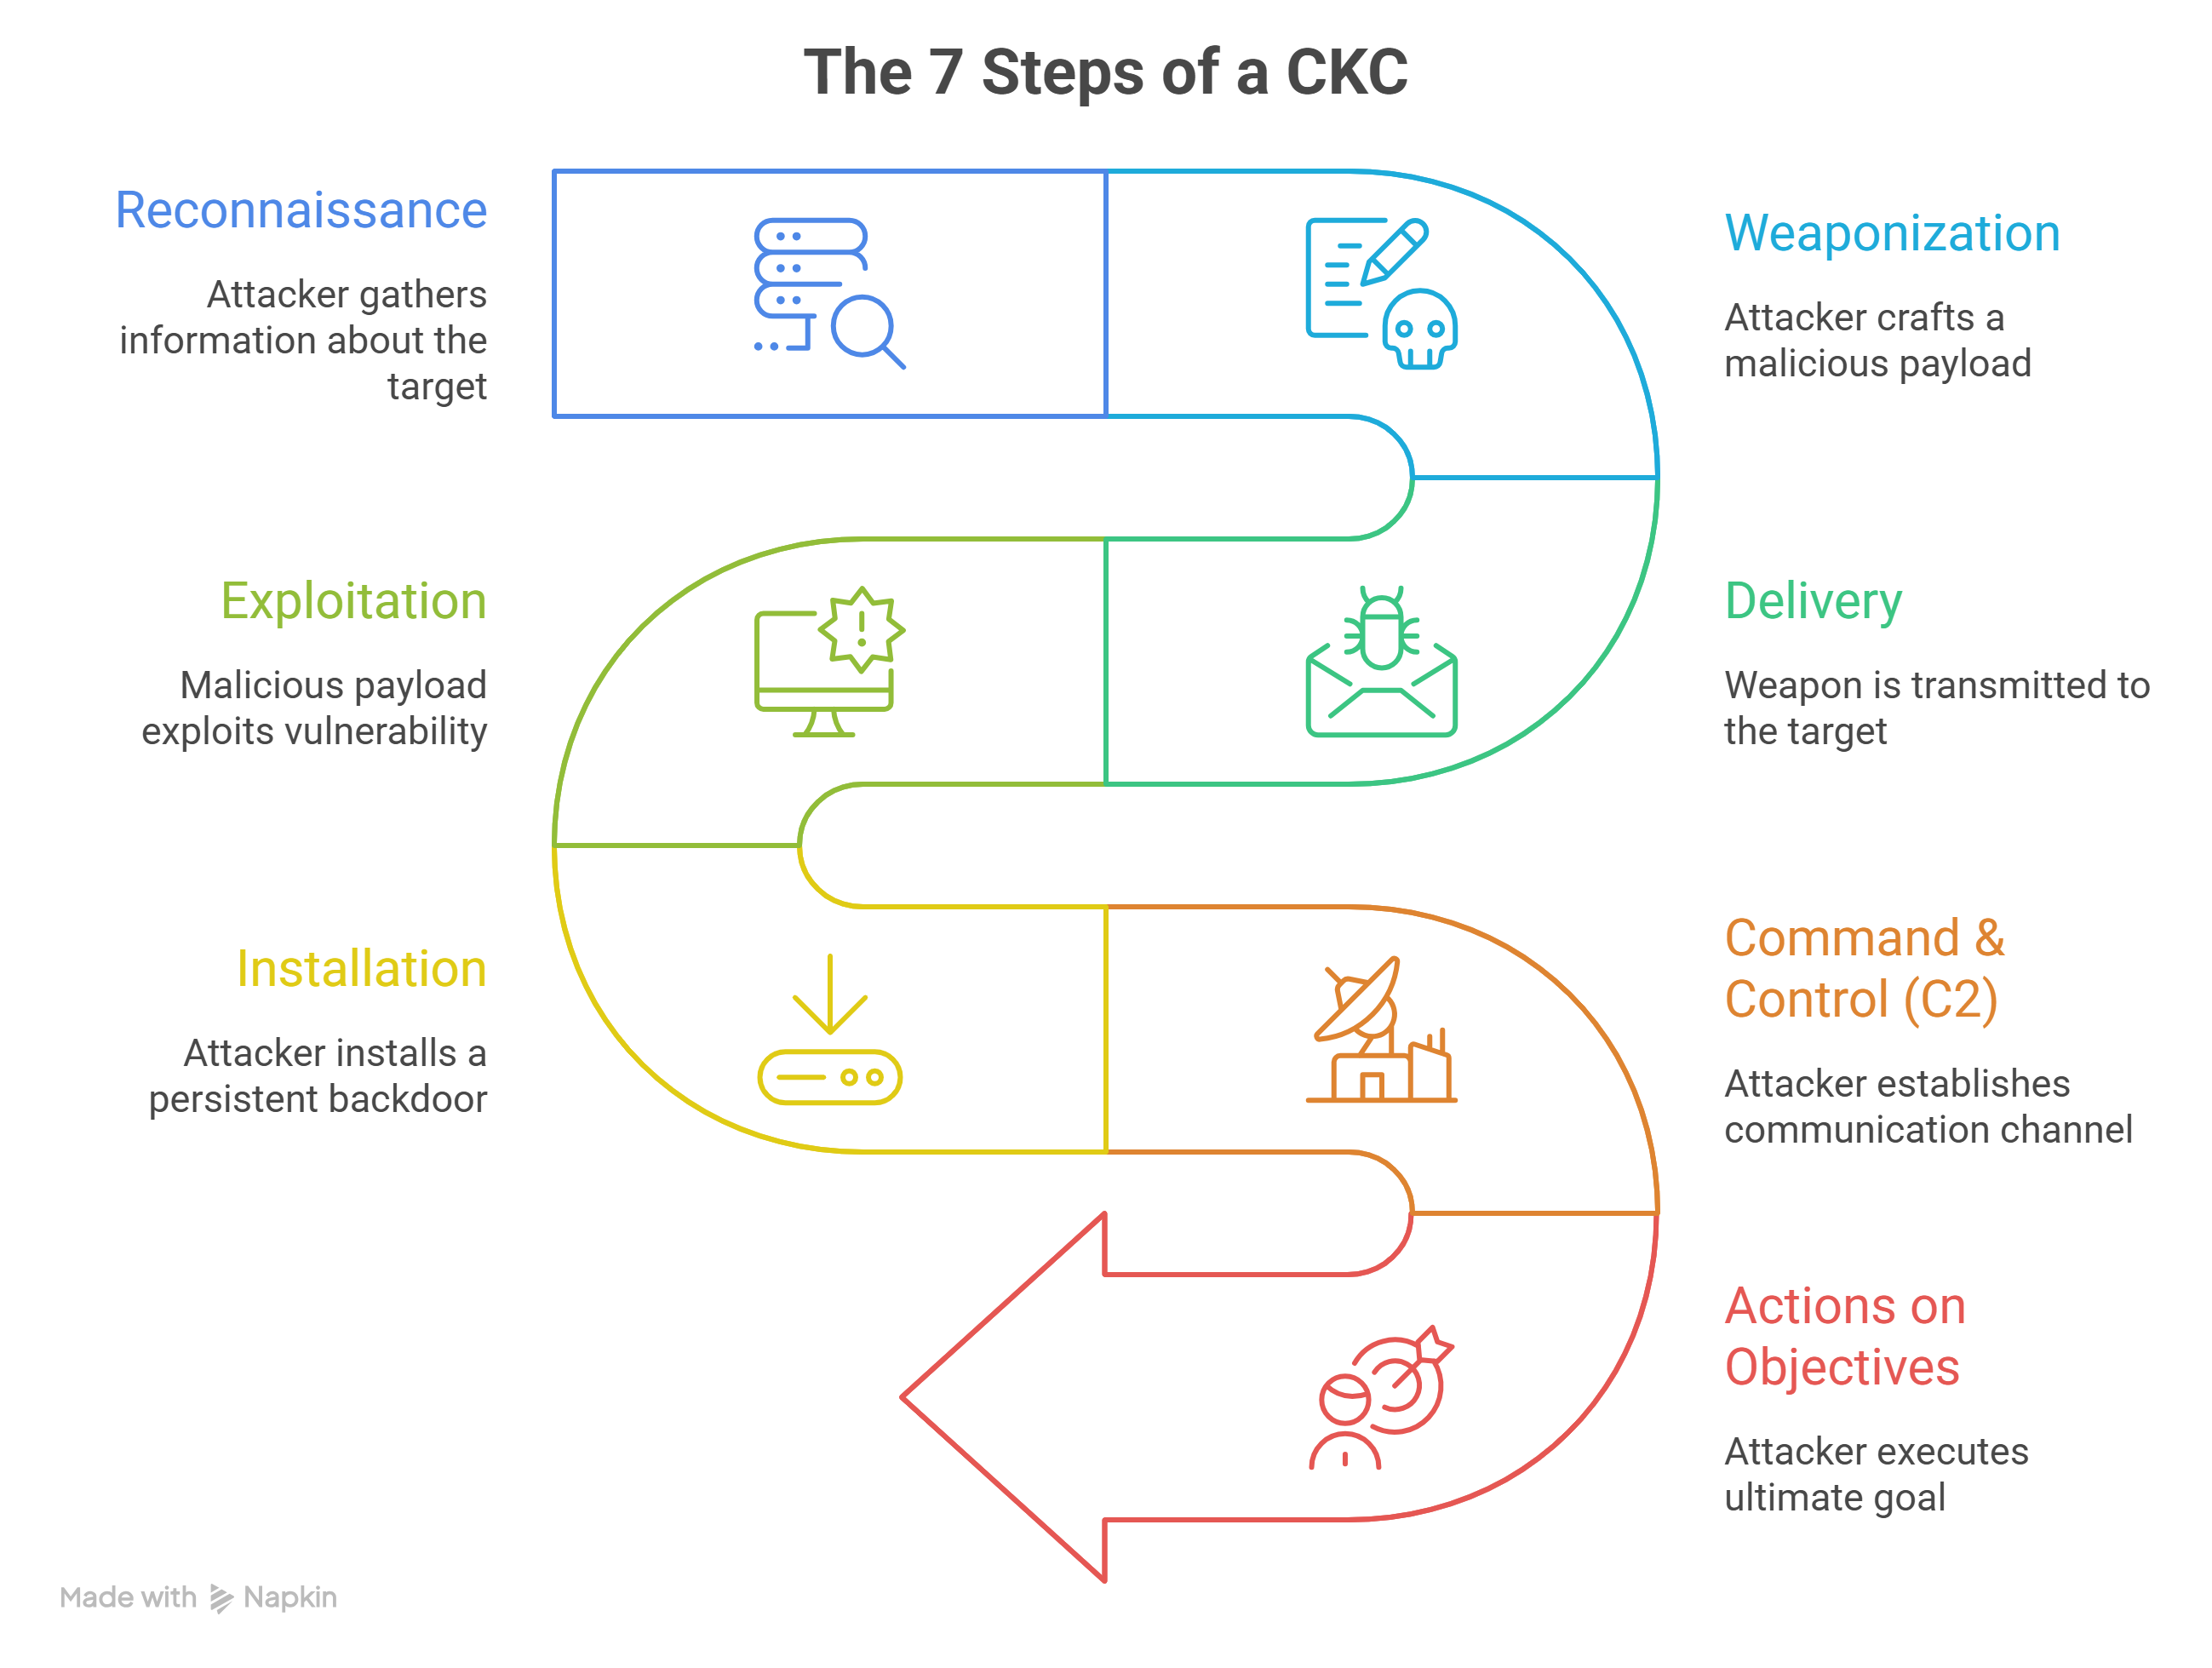
\includegraphics[width=0.9\textwidth]{figures/ch1/the_7_steps_ckc.png}
    \caption{The 7 Steps of the Cyber Kill Chain (CKC)}
    \label{fig:ckc_7steps}
\end{figure}

\section{The MITRE ATT\&CK Framework}
\subsection{Fundamental Concepts and Structure}
MITRE ATT\&CK (Adversarial Tactics, Techniques, and Common Knowledge) is a structured knowledge base describing cyber adversary behavior across various domains (enterprise, mobile, industrial control systems - ICS) \cite{jiang2025mitre}. Developed in 2013, it serves as a fundamental basis for mapping adversary Tactics, Techniques, and Procedures (TTPs) \cite{jiang2025mitre}.

The framework's structure revolves around four main components \cite{jiang2025mitre}:
\begin{enumerate}
    \item \textbf{Tactics}: The adversary's high-level objectives (similar to CKC phases, but more numerous and detailed).
    \item \textbf{Techniques}: The specific methods used to achieve these objectives.
    \item \textbf{Sub-techniques}: Detailed methods that break down techniques.
    \item \textbf{Documented Usage}: Associated procedures and metadata.
\end{enumerate}
ATT\&CK is organized into matrices representing adversary operating environments: \textbf{Enterprise} (traditional networks and cloud), \textbf{Mobile}, and \textbf{ICS} \cite{jiang2025mitre}.

\begin{figure}[H]
    \centering
    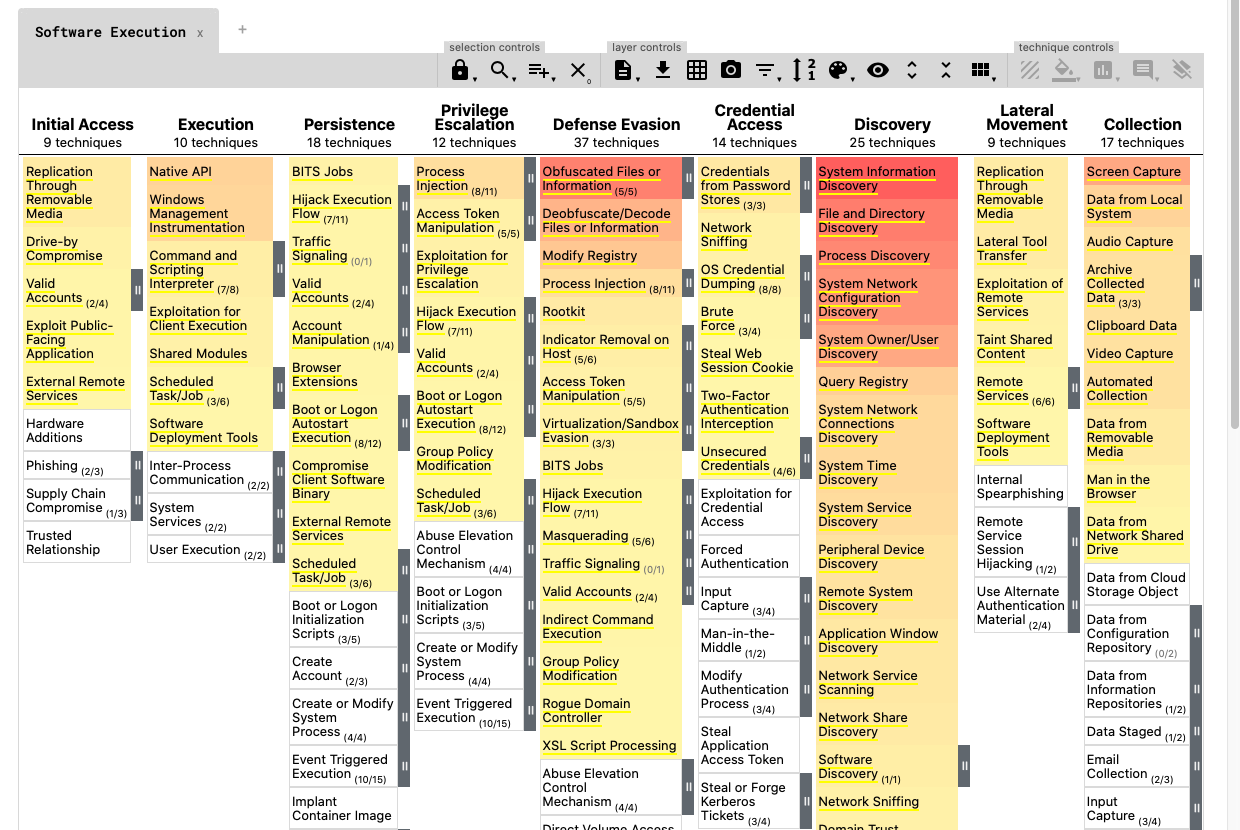
\includegraphics[width=0.9\textwidth]{figures/ch1/MITRE.png}
    \caption{The MITRE ATT\&CK Framework matrix}
    \label{fig:mitre_framework}
\end{figure}

\subsection{Applications and Integration with CKC}
MITRE ATT\&CK is a widely adopted tool for strengthening cybersecurity, notably by supporting Cyber Threat Intelligence (CTI), incident response, attack modeling, and vulnerability prioritization \cite{jiang2025mitre}.

\textbf{APT Detection}: One of the fundamental uses of ATT\&CK is improving the systematic detection and analysis of threats, particularly APTs \cite{jiang2025mitre}. The framework is used to model APT attack footprints using TTP-based attack trees. Coverage percentage relative to ATT\&CK is even used as a metric to evaluate the performance of APT detection models\footnote{\textbf{What is ATT\&CK Coverage Percentage as a Metric?} When researchers build an APT detection model, they measure how many ATT\&CK techniques their model can detect. The coverage percentage tells you: "Out of all the known attack techniques in the ATT\&CK framework, how many can this model catch?" � a higher percentage means the model is better at detecting a wider range of attacks.}. Studies identify that the most frequently observed tactics are Initial Access (especially Spearphishing Link at 45.5\%), Execution, and Discovery \cite{jiang2025mitre, cisa202x}.

\textbf{CKC/ATT\&CK Integration}: ATT\&CK is often integrated with other frameworks like the Cyber Kill Chain. While CKC offers a sequential view of the attack, ATT\&CK provides the granularity of TTPs at each stage \cite{jiang2025mitre}. Integration fills the gaps in CKC, which lacks detailed information on adversary tactics and techniques. This complementarity is vital for early detection, as it maps adversary actions to different CKC phases \cite{jiang2025mitre}.

\customexplication{If the Kill Chain provides the chapter headings, ATT\&CK provides the detailed content for each chapter.}

\section{Introduction to Machine Learning}

\subsection{Definition and Core Concepts of Machine Learning}

Machine Learning (ML) is a subfield of Artificial Intelligence (AI) that enables computer systems to learn from data and improve their performance on a given task without being explicitly programmed to do so~\cite{bishop2006pattern}. Rather than following a fixed set of rules written by a programmer, an ML model identifies patterns, relationships, and regularities within data, and uses this learned knowledge to make predictions or decisions on new, unseen data.

Formally, the learning process can be described as follows: given a set of training examples, an ML algorithm adjusts its internal parameters to minimize the difference between its predictions and the actual outcomes~\cite{bishop2006pattern} --- a process known as optimization. The quality of this learning is measured using a loss function, which quantifies how far the model's predictions are from the true values.


\customexplication{A helpful analogy: teaching a child to recognize cats does not involve giving them a precise list of rules (``four legs, pointed ears, fur''). Instead, you show them hundreds of examples of cats and non-cats, and they gradually learn to distinguish them on their own. Machine Learning works in exactly the same way --- it learns from examples rather than from explicit instructions.}

\subsubsection*{Core Concepts}

\begin{description}
    \item[Training Data] The dataset used to teach the model. It consists of input examples (features) and, in supervised settings, their corresponding correct outputs (labels). The quality, quantity, and diversity of training data directly determine the quality of the learned model.
    
    \item[Features] The individual measurable properties or characteristics of the data used as inputs to the model. Feature selection and engineering --- the process of choosing and transforming the most relevant features --- is one of the most critical steps in building an effective ML model.
    
    \item[Model] A mathematical function or structure that maps input data to an output prediction. The model's internal parameters are adjusted during training to best fit the patterns observed in the training data.
    
    \item[Training and Testing] The dataset is typically split into:
    \begin{itemize}
        \item \textbf{Training set}: Used to fit the model's parameters.
        \item \textbf{Validation set}: Used to tune hyperparameters and monitor learning during training.
        \item \textbf{Test set}: Used to evaluate the model's final performance on completely unseen data.
    \end{itemize}
    
    \item[Overfitting and Underfitting] Two fundamental challenges in ML model development~\cite{hastie2009elements}:
    \begin{itemize}
        \item \textbf{Overfitting} occurs when a model learns the training data too well --- including its noise and irrelevant details --- resulting in poor generalization to new data.
        \item \textbf{Underfitting} occurs when a model is too simple to capture the underlying patterns in the data, resulting in poor performance on both training and test data. These concepts are visually illustrated in Figure~\ref{fig:over_under}.
    \end{itemize}

\begin{figure}[H]
    \centering
    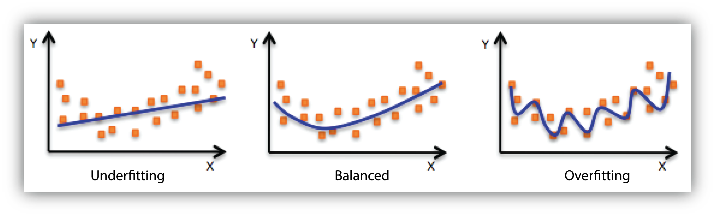
\includegraphics[width=0.8\textwidth]{figures/ch1/over_under.png}
    \caption{Visual representation of Underfitting, Optimal Fit, and Overfitting.}
    \label{fig:over_under}
\end{figure}
    
  \customwarning{Overfitting is a particularly significant concern in cybersecurity applications of ML, where models must generalize to novel, previously unseen attack patterns rather than simply memorizing known ones (which would essentially reduce the ML model into a traditional signature-based detection system).}
    
    \item[Hyperparameters] Configuration settings defined before training begins --- such as learning rate\footnote{The learning rate is a parameter that dictates the step size at each iteration while the machine learning algorithm attempts to minimize the loss function.}, number of layers, or number of trees --- that control the learning process itself, as opposed to the model parameters learned from data.
    
    \item[Generalization] The ability of a trained model to perform well on new, unseen data that was not part of the training set~\cite{hastie2009elements}. Generalization is the ultimate goal of any ML model, and is especially critical in dynamic environments such as cybersecurity, where threat patterns evolve continuously.
    
    \item[Loss Function and Optimization] The loss function measures how far the model's predictions deviate from the true labels. The training process seeks to minimize this loss using optimization algorithms --- the most common being Gradient Descent and its variants (e.g., Adam, SGD), which iteratively adjust model parameters in the direction that reduces the loss~\cite{goodfellow2016deep}.
    
    \item[Evaluation Metrics] Once trained, a model's performance is assessed using metrics appropriate to the task:
    \begin{itemize}
        \item \textbf{Accuracy}: The proportion of correct predictions out of all predictions.
        \item \textbf{Precision}: The proportion of true positive predictions among all positive predictions.
        \item \textbf{Recall (Sensitivity)}: The proportion of actual positives correctly identified by the model.
        \item \textbf{F1-Score}: The harmonic mean of precision and recall, balancing both metrics.
        \item \textbf{AUC-ROC}: A measure of the model's ability to distinguish between classes across all classification thresholds~\cite{fawcett2006roc}.
    \end{itemize}
\end{description}

\customexplication{
In the context of cybersecurity and attack detection, the evaluation metrics are based on four possible outcomes, where the "Positive" class typically represents an \textit{attack} or anomaly, and the "Negative" class represents \textit{normal/benign} behavior:
\begin{itemize}
    \item \textbf{True Positive (TP)}: The model correctly identifies an \textit{actual attack}. This is a successful detection.
    \item \textbf{True Negative (TN)}: The model correctly identifies \textit{normal activity}. This is a successful passing of safe traffic.
    \item \textbf{False Positive (FP)}: The model incorrectly flags \textit{normal activity as an attack} (a false alarm).
    \item \textbf{False Negative (FN)}: The model incorrectly identifies an \textit{attack as normal activity}. This is a critical failure where the threat slips through.
\end{itemize}
}

\customnote{In cybersecurity and APT detection specifically, \textbf{Recall} is often prioritized over \textbf{Accuracy}. Missing a real attack (a false negative) is far more costly than incorrectly flagging a benign event (a false positive). A model that detects 99\% of attacks while generating some false alarms is far preferable to one that misses critical threats.}

Machine Learning's ability to detect complex, non-linear patterns in large datasets makes it particularly well-suited for cybersecurity applications~\cite{buczak2016survey} --- a capability that static, rule-based systems fundamentally lack. The following sections elaborate on the different learning paradigms ML employs, and on how these capabilities are used to detect sophisticated threats such as APTs.

\subsection{Domains and Learning Paradigms}

Machine Learning is not a single, uniform approach --- it includes several distinct learning paradigms, each defined by the type of data available and the nature of the task to be solved. Understanding these paradigms is essential, as different cybersecurity problems require different learning strategies. Additionally, ML operates across a range of application domains, each contributing specific capabilities to threat detection and analysis, as illustrated in Figure~\ref{fig:ml_domain}.

\begin{figure}[H]
    \centering
    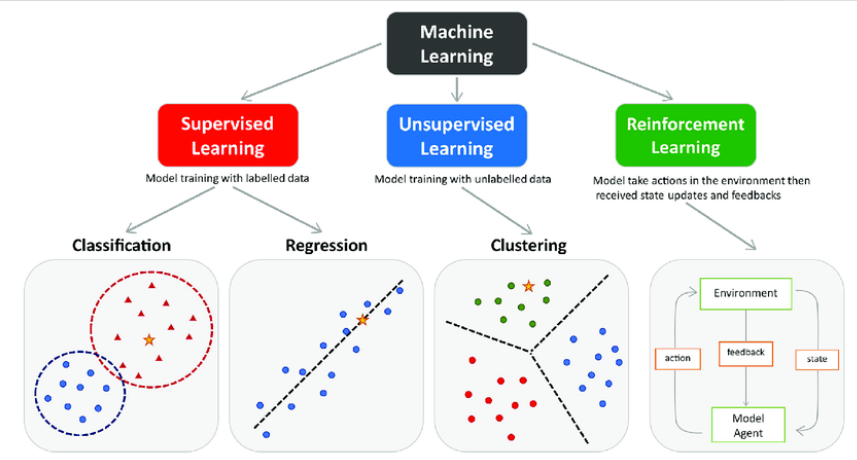
\includegraphics[width=0.8\textwidth]{figures/ch1/ml_domain.png}
    \caption{Machine Learning domains and learning paradigms.}
    \label{fig:ml_domain}
\end{figure}

\subsubsection*{Learning Paradigms}

\begin{description}
    \item[Supervised Learning] Supervised learning is the most widely used ML paradigm. The model is trained on a labeled dataset --- meaning each input example is paired with a known, correct output (label). The model learns to map inputs to outputs by minimizing the error between its predictions and the true labels.
    \begin{itemize}
        \item \textbf{Task types}: Classification (assigning a category) and Regression (predicting a continuous value).
        \item \textbf{Common algorithms}: Decision Trees, Random Forests, Support Vector Machines (SVM), Logistic Regression, Neural Networks.
        \item \textbf{Cybersecurity application}: Classifying network traffic as malicious or benign, detecting known malware families, identifying phishing emails~\cite{buczak2016survey}.
    \end{itemize}
    
\customexplication{Supervised learning is analogous to studying with an answer key --- the model sees both the questions (inputs) and the correct answers (labels) during training, and learns to produce correct answers on new questions it has never seen before.}

    \item[Unsupervised Learning] In unsupervised learning, the model is trained on unlabeled data --- no predefined correct outputs are provided. The model must discover hidden structure, patterns, or groupings within the data on its own~\cite{chandola2009anomaly}.
    \begin{itemize}
        \item \textbf{Task types}: Clustering (grouping similar examples) and Dimensionality Reduction (simplifying data representation while preserving key information).
        \item \textbf{Common algorithms}: K-Means, DBSCAN, Hierarchical Clustering, Principal Component Analysis (PCA).
    \end{itemize}
    

    \item[Semi-Supervised Learning] Semi-supervised learning operates with a partially labeled dataset --- a small amount of labeled data combined with a large amount of unlabeled data. The model leverages both to improve learning performance beyond what would be achievable with labeled data alone~\cite{zhu2005semisupervised}.
    \begin{itemize}
        \item \textbf{Why it matters}: Obtaining large quantities of labeled cybersecurity data is expensive and time-consuming, as labeling requires expert knowledge. Semi-supervised learning addresses this practical limitation~\cite{zhu2005semisupervised}.
        \item \textbf{Common approaches}: Self-training, Label Propagation, Generative Adversarial Networks (GANs) for data augmentation.
        \item \textbf{Cybersecurity application}: Training APT detection models when only a small number of confirmed attack samples are available, augmented by large volumes of unlabeled network logs.
    \end{itemize}
    

    \item[Reinforcement Learning (RL)] Reinforcement Learning is a paradigm in which an agent learns to make sequential decisions by interacting with an environment. The agent receives a reward or penalty based on the outcome of each action, and gradually learns a policy --- a strategy for choosing actions --- that maximizes cumulative reward over time~\cite{sutton2018reinforcement}.
    \begin{itemize}
        \item \textbf{Key components}: Agent, Environment, State, Action, Reward, Policy.
        \item \textbf{Common algorithms}: Q-Learning, Deep Q-Networks (DQN), Proximal Policy Optimization (PPO)~\cite{sutton2018reinforcement}.
    \end{itemize}
    
\end{description}

\subsubsection*{ML Application Domains}

Beyond learning paradigms, ML operates across several technical domains, each providing distinct capabilities relevant to cybersecurity:

\begin{table}[h]
\centering
\caption{Key Machine Learning Application Domains in Cybersecurity}
\label{tab:ml_domains}
\begin{tabular}{|p{0.25\linewidth}|p{0.35\linewidth}|p{0.35\linewidth}|}
\hline
\textbf{Domain} & \textbf{Description} & \textbf{Cybersecurity Application} \\ \hline
Natural Language Processing (NLP) & Processing and understanding human language text & Extracting TTPs from threat intelligence reports, detecting phishing content \\ \hline
Anomaly Detection & Identifying data points that deviate significantly from expected patterns & Detecting unusual network behavior, insider threats, APT lateral movement \\ \hline
Time Series Analysis & Modeling sequential, time-ordered data & Detecting multi-stage APT attack sequences across time \\ \hline
Graph Learning & Analyzing relationships and connections between entities & Mapping attacker infrastructure, detecting lateral movement paths \\ \hline
Generative AI (GenAI) & Generating new data samples similar to training data & Synthetic attack data generation, CTI report summarization, threat simulation \\ \hline
\end{tabular}

\end{table}

\textbf{Choosing the Right Paradigm:}
The choice of learning paradigm depends on the nature of the available data and the detection objective:
\begin{itemize}
    \item When labeled attack data is available $\rightarrow$ \textbf{Supervised Learning}
    \item When only raw, unlabeled logs are available $\rightarrow$ \textbf{Unsupervised Learning}
    \item When limited labels exist within large unlabeled datasets $\rightarrow$ \textbf{Semi-Supervised Learning}
    \item When the system must adapt dynamically to evolving threats $\rightarrow$ \textbf{Reinforcement Learning}
\end{itemize}

\customnote{ In practice, state-of-the-art APT detection systems rarely rely on a single paradigm. The most effective approaches --- including those proposed in Chapter 3 --- combine multiple paradigms: using unsupervised methods for anomaly detection, supervised models for TTP classification, and reinforcement learning for adaptive, multi-stage response.}

\clearpage

